\chapter{Понятие цифровых моделей местности и их классификация}

Цифровая модель местности (ЦММ) – это множество элементов, являющиеся топографо-геодезической информацией о местности.
ЦММ включает в себя: 

\begin{enumerate} 
  \item[1)] метрическую информацию о геодезических пространственных координатах характерных точек рельефа и ситуации;
  
  \item[2)] синтаксическую информацию, используемую для описания связей между точками границ зданий, лесов, водоемов, дорог, водораздельных и водосливных линии и т.п.;
  
  \item[3)] семантическую информацию, характеризующую свойства объектов, а именно технические параметры инженерных сооружений, геологические характеристики грунтов, данные о деревьях в лесных массивах и т.п.;
  
  \item[4)] структурную информацию, описывающую связи между различными объектами, отношения объектов к какому-либо множеству, например, раздельные пункты железнодорожной линии, здания и сооружения населенного пункта, строения и конструкции производств и т.п.;
  
  \item[5)] общую информацию, это может быть название участка, система координат и высот, номенклатура \cite{19,10}.
  
\end{enumerate} 


ЦММ характеризует ситуацию и рельеф местности. Она состоит из цифровой модели рельефа (ЦМР) и цифровой модели контуров (ЦМК). Кроме этого ЦММ может дополняться моделью специального инженерного назначения (ЦМИН) \cite{11}.

\section{Цифровые модели рельефа}

Цифровая модель рельефа представляет собой поверхность местности, которая не включает в себя объекты, находящиеся на поверхности, которая создается на основе данных о высоте. Поверхность местности может быть представлена как трехмерная (3D) или двумерная (2D) \cite {1, 23}.

Источники для исходных данных для построения ЦМР очень разнообразны: 

\begin{enumerate} 
  \item[1)] радарная топографическая съемка местности;
  \item[2)] методы кинематической глобальной навигационной спутниковой системы;
  \item[3)] данные дистанционного зондирования Земли;
  \item[4)] материалы полевых съемок;
  \item[5)] методы определения структуры по движению;
  \item[6)] интерполяция цифровых контурных карт или данных из прямых съемок поверхности земли и другие \cite{2, 17}.
\end{enumerate} 

С помощью ЦМР можно автоматически извлечь морфометрические данные, такие как уклоны и изломы, аспект уклона, альтиметрические пояса, шероховатость или зернистость поверхности, а также параметры, касающиеся гидрографических сетей. Также при использовании ЦМР можно решить задачи связанные с оценкой форм склонов, через кривизну их поперечного сечения, проведением интерполяции по значениям высот, проведением трехмерной визуализации рельефа, проведением оценки видимости или невидимости  с определенной точки обзора и многие другие \cite{15,13}.

Существуют определенные требования, которым цифровая модель рельефа должна соответствовать:

\begin{enumerate} 
  \item[1)] модель должна содержать в себе доступную информацию, которую получают в результате наблюдений;
  \item[2)] параметры, которые присущи модели, должны иметь однозначный физический смысл и возможность прямого измерения;
  \item[3)] систематизация значений параметров позволит использовать их при моделировании стока в малоизученных бассейнах \cite{3,21}.
\end{enumerate} 

Также модель рельефа может быть представленна как матрица высот или матрица качеств.

\subsection{Матрицы высот рельефа местности}

Матрица высот может быть построена по тем данным объектов карты рельефа местности, которые имеют абсолютную высоту или 3D-метрику. В задачах анализа рельефа, которых касаются построения профилей и зон видимости, а также в задачах вычисления площади или длины объекта с учетом рельефа такая матрица высот может использоваться в качестве основы. Также в задачах моделирования зон затопления, формирования объемной карты местности, определения направления склонов и других \cite{4,12}.

\begin{figure}[h!]
    \center
    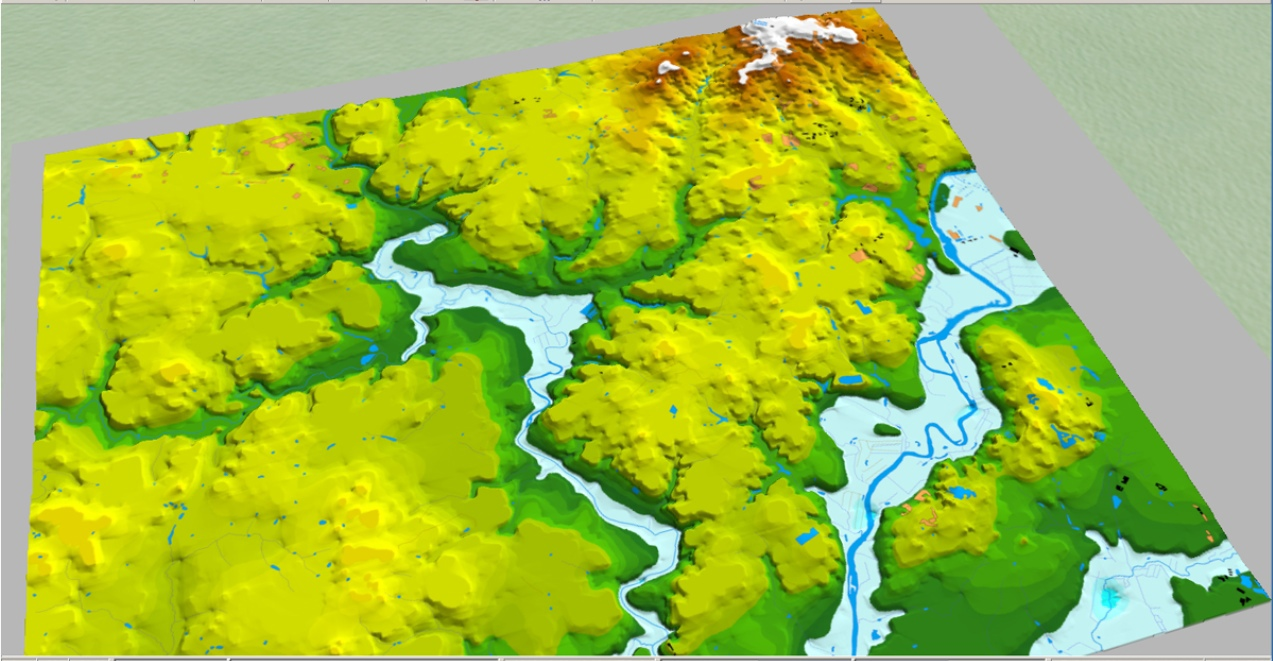
\includegraphics[scale=0.3]{images/112.jpg}
    \caption{Пример матрицы высот}
    \label{fig:1}
\end{figure}

Для формирования трехмерной метрики определенных объектов, содержащихся на карте, или для получения отмывки рельефа в виде растрового изображения, оценки и анализа статистики поверхности указанного участка местности, а также для создания автоматического построения изолиний -- используют матрицу высот рельефа \cite{5,14}. Пример матрицы высот изображен на рисунке
\ref{fig:1}.

\subsection{Использование матриц качеств для характеристик поверхности}

Обычно матрицу качеств представляют в виде поверхности значений определенной моделируемой характеристики. Для построения матрицы качеств могут использоваться значения смысловой характеристики объектов, содержащиеся на векторной карте или в выбранных полях таблицы базы данных \cite{6, 7}. 

Данные, которые может содержать матрица качеств очень различны. Это может быть, как тип растительности или землевладения, плотность застройки, так и качественные характеристики почвы, глубина залегания грунтовых вод, концентрация выхлопных газов и т.д.

Модель поверхности, которая представлена матрицей качеств, можно изменить, выполняя определенные операции (арифметические и логические) над её элементами. Используя матрицу качеств можно осуществить анализ определенной моделируемой характеристики с помощью поиска областей, значения характеристики в которых удовлетворяют набору заданных условий. Результаты такого анализа могут сохранятся в двух видах -- растрового изображения или матрицы качеств \cite{8,16}. Пример матрицы качеств изображен на рисунке \ref{fig:2}.

\begin{figure}[h!]
    \center
    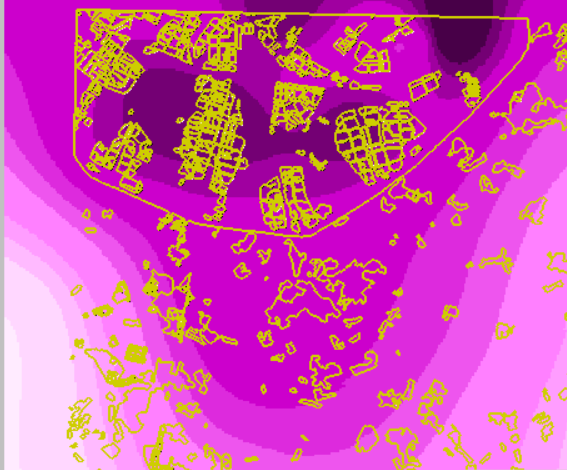
\includegraphics[scale=0.7]{images/111.png}
    \caption{Пример матрицы качеств концентрации выхлопных газов}
    \label{fig:2}
\end{figure}

\subsection{Классификация цифровых моделей рельефа}
Классифицировать ЦМР можно по нескольким признакам, например по характеру нахождения объектов: регулярные и нерегулярные.

В регулярных ЦМР заметно, что точки моделирующие поверхность земли находятся в пересечении узлов сетки, которую проецируют на местность. В подобной сетке форма ячеек может являться различными геометрическими объектами: прямоугольники, квадраты, равносторонние треугольники (рисунок ~\ref{fig:3}).

\begin{figure}[h!]
    \center
    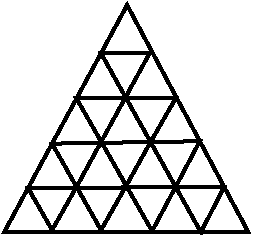
\includegraphics[scale=2]{images/regular.png}
    \caption{Пример регулярной сетки}
    \label{fig:3}
\end{figure}

Такая ЦМР наиболее проста, так как легче провести ее построение, особенно если в районе, в котором строится ЦМР, проводились геодезические работы \cite{9,20}. 

Эффективность, достигаемая в условиях однородной местности или городской застройки, является достойным преимуществом регулярной ЦМР.

Основными минусами регулярной ЦМР являются:  

\begin{enumerate} 
  \item[1)] ключевые точки рельефа, такие как вершины, впадины, глубины, границы оврагов и т.п., не всегда  совпадают с узлами сетки;
  \item[2)] регулярные ЦМР требуют много трудозатрат при разбиении узловых точек на местности и определении значений высоты в каждой из них;
  \item[3)] при резко меняющемся рельефе, особенно если размеры ячеек очень большие, значительная часть информации может не отразиться в ЦМР (например овраги);
  \item[4)] при слишком маленьких размерах ячеек на достаточно однородной части рельефа, может случиться переизбыток точек, будет занят довольно большой объем памяти и потребуются лишние затраты времени и труда на ввод отметок высоты в узлах сетки \cite{19,22}.
\end{enumerate} 

Регулярные модели нашли применение при проектировани аэродромов, городских улиц, при вертикальной планировке, то есть тогда, когда требуется повышенная детальность исходной информации. 

Также существуют нерегулярные ЦМР, в которых точки размещаются в произвольном порядке, но при этом с заданной частотой и плотностью. Чем сложнее рельеф на местности, тем гуще должна быть построенная сетка (рисунок~\ref{fig:4}). Такая ЦМР позволяет ввести все ключевые точки рельефа~\cite{10}.

Одним из видов нерегулярной сетки является образующаяся при сканировании различных топографических материалов сетка.

У ЦМР, построенной на основе такой сетки, также имеется недостаток~--~для каждой точки необходимо вводить ее номер, координаты $x$, $y$ и отметки высот $h$.

После того как ключевые точки рельефа нерегулярной сетки будут отображены на карту, по данным этих точек будет строиться модель поверхности одним из существующих методов \cite{11,18}. 

\begin{figure}[h!]
    \center
    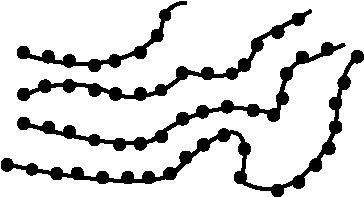
\includegraphics[scale=2.5]{images/unregular.png}
    \caption{Пример нерегулярной сетки}
    \label{fig:4}
\end{figure}

\section{Цифровая модель контуров}

Цифровая модель контуров, также называемая цифровой моделью ситуации, состоит из совокупности точечных, линейных и площадных топографических объектов, с заданными координатами принадлежащих им точек и семантической информацией в виде списка характеристик, значения которых можно изменять. 

Семантика ЦМК имеет влияние на представление элемента в разных видах, таких как план, профиль, сечение, 3D-вид. Атрибуты должны определять как качественные параметры, например, треугольная труба или шестиугольная в сечении, тропическое растение или лиственное, так и количественные параметры объектов, например, длина, площадь. Связи таких атрибутов между собой определяют не только вид, но и поведение элемента в разных ситуациях и проекциях \cite{18,20}.

На рисунке \ref{fig:5} представлена цифровая модель контуров. Точки контуров (углы зданий, углы поворота линейных объектов и т.д.) определяют значения координат $X$ и $Y$ без значения высоты $H$. Также указана взаимосвязь точек контура, например, группа точек (1,2,3,4) определяет сплошной контур жилого дома, а группа точек (15,16,17,18) определяет контур дороги.

\begin{figure}[h!]
    \center
    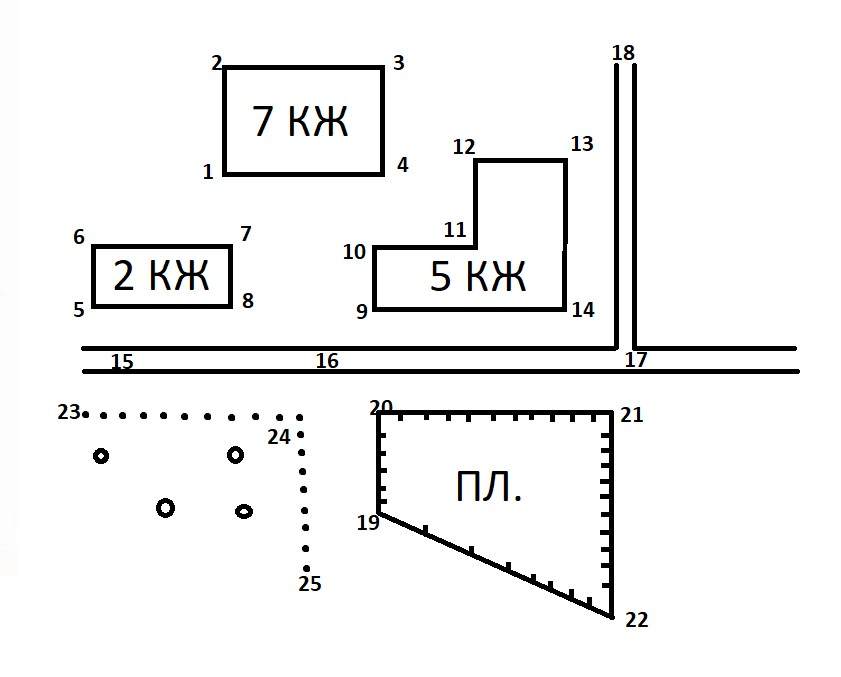
\includegraphics[scale=0.52]{images/1717.jpg}
    \caption{Пример цифровой модели контуров}
    \label{fig:5}
\end{figure}

\section{Цифровые модели специального инженерного назначения}

Цифровые модели специального инженерного назначения широко используются в виде результатов инженерно-геодезических изысканий. Проектировщику нужно принимать определенные решения, которые касаются решений по проекту, пользуясь в качестве исходных данных физическим состоянием определенной местности. Это требует, кроме соблюдения норм инженерно-геодезических изысканий, таких как состав, полнота данных, точность, еще и таких условий как: 

\begin{enumerate} 
  \item[1)] соответствие ЦМР её топографической реальности;
  \item[2)] пространственного представления в модели подземных и надземных коммуникаций;
  \item[3)] многослойности модели рельефа и ситуации с заданным распределением данных, необходимых проектировщику, по отдельно организованным слоям;
   \item[4)] информационной насыщенности объектов модели сведениями, необходимыми для принятия проектных решений и согласований \cite{22}.
\end{enumerate} 

\section{Классификация цифровых моделей местности}

ЦММ полностью соответствуют классификации карт по назначению, а именно топографические, контурные, геологические, кадастровые и др.

Цифровые модели местности делятся на четыре типа по способу размещения их исходной информации и правил ее обработки на электронно-вычислительной машине (ЭВМ). 

\begin{enumerate} 
  \item[1.] Регулярные, в которых опорные точки с известными координатами располагаются в узлах геометрических сеток различной формы (рисунок~\ref{fig:6}~а) регулярная сетка ЦММ). Такие используют для равнинной местности.
 
  \item[2.] Нерегулярные, в которых точки располагаются произвольно в пределах однородных по рельефу, геологии, гидрологии участков местности без какой-либо определенной системы, но с заданной густотой и плотностью (рисунок~\ref{fig:6}~б) нерегулярная сетка ЦММ).

  \item[3.] Структурные, в которых точки с известными координатами расставлены в вершинах переломов структурных (орографических) линий рельефа. Точки таких ЦММ могут распологаться на основных перегибах всех структурных линий: рисунок~\ref{fig:7}~(а)~--~ структурная сетка, точки которой располагаются вдоль скатов в местах изменения кривизны склонов, рисунок~\ref{fig:7}~(б)~--~ структурная сетка, точки которой расположены на основных перегибах, вдоль скатов по линии наибольшей крутизны в местах характерных переломов с указанием крутизны и направлений линий, рисунок~\ref{fig:7}~(в)~--~структурная сетка, точки которой расположены в местах изменения кривизны склонов. Структурные ЦММ используют для пересеченной местности.

   \item[4.] Статические -- основаны на определении координат точек, случайно и часто выбранных на местности~\cite{23}.
\end{enumerate} 

 \begin{figure}[h]
    \begin{minipage}[h]{0.5\linewidth}
    \center{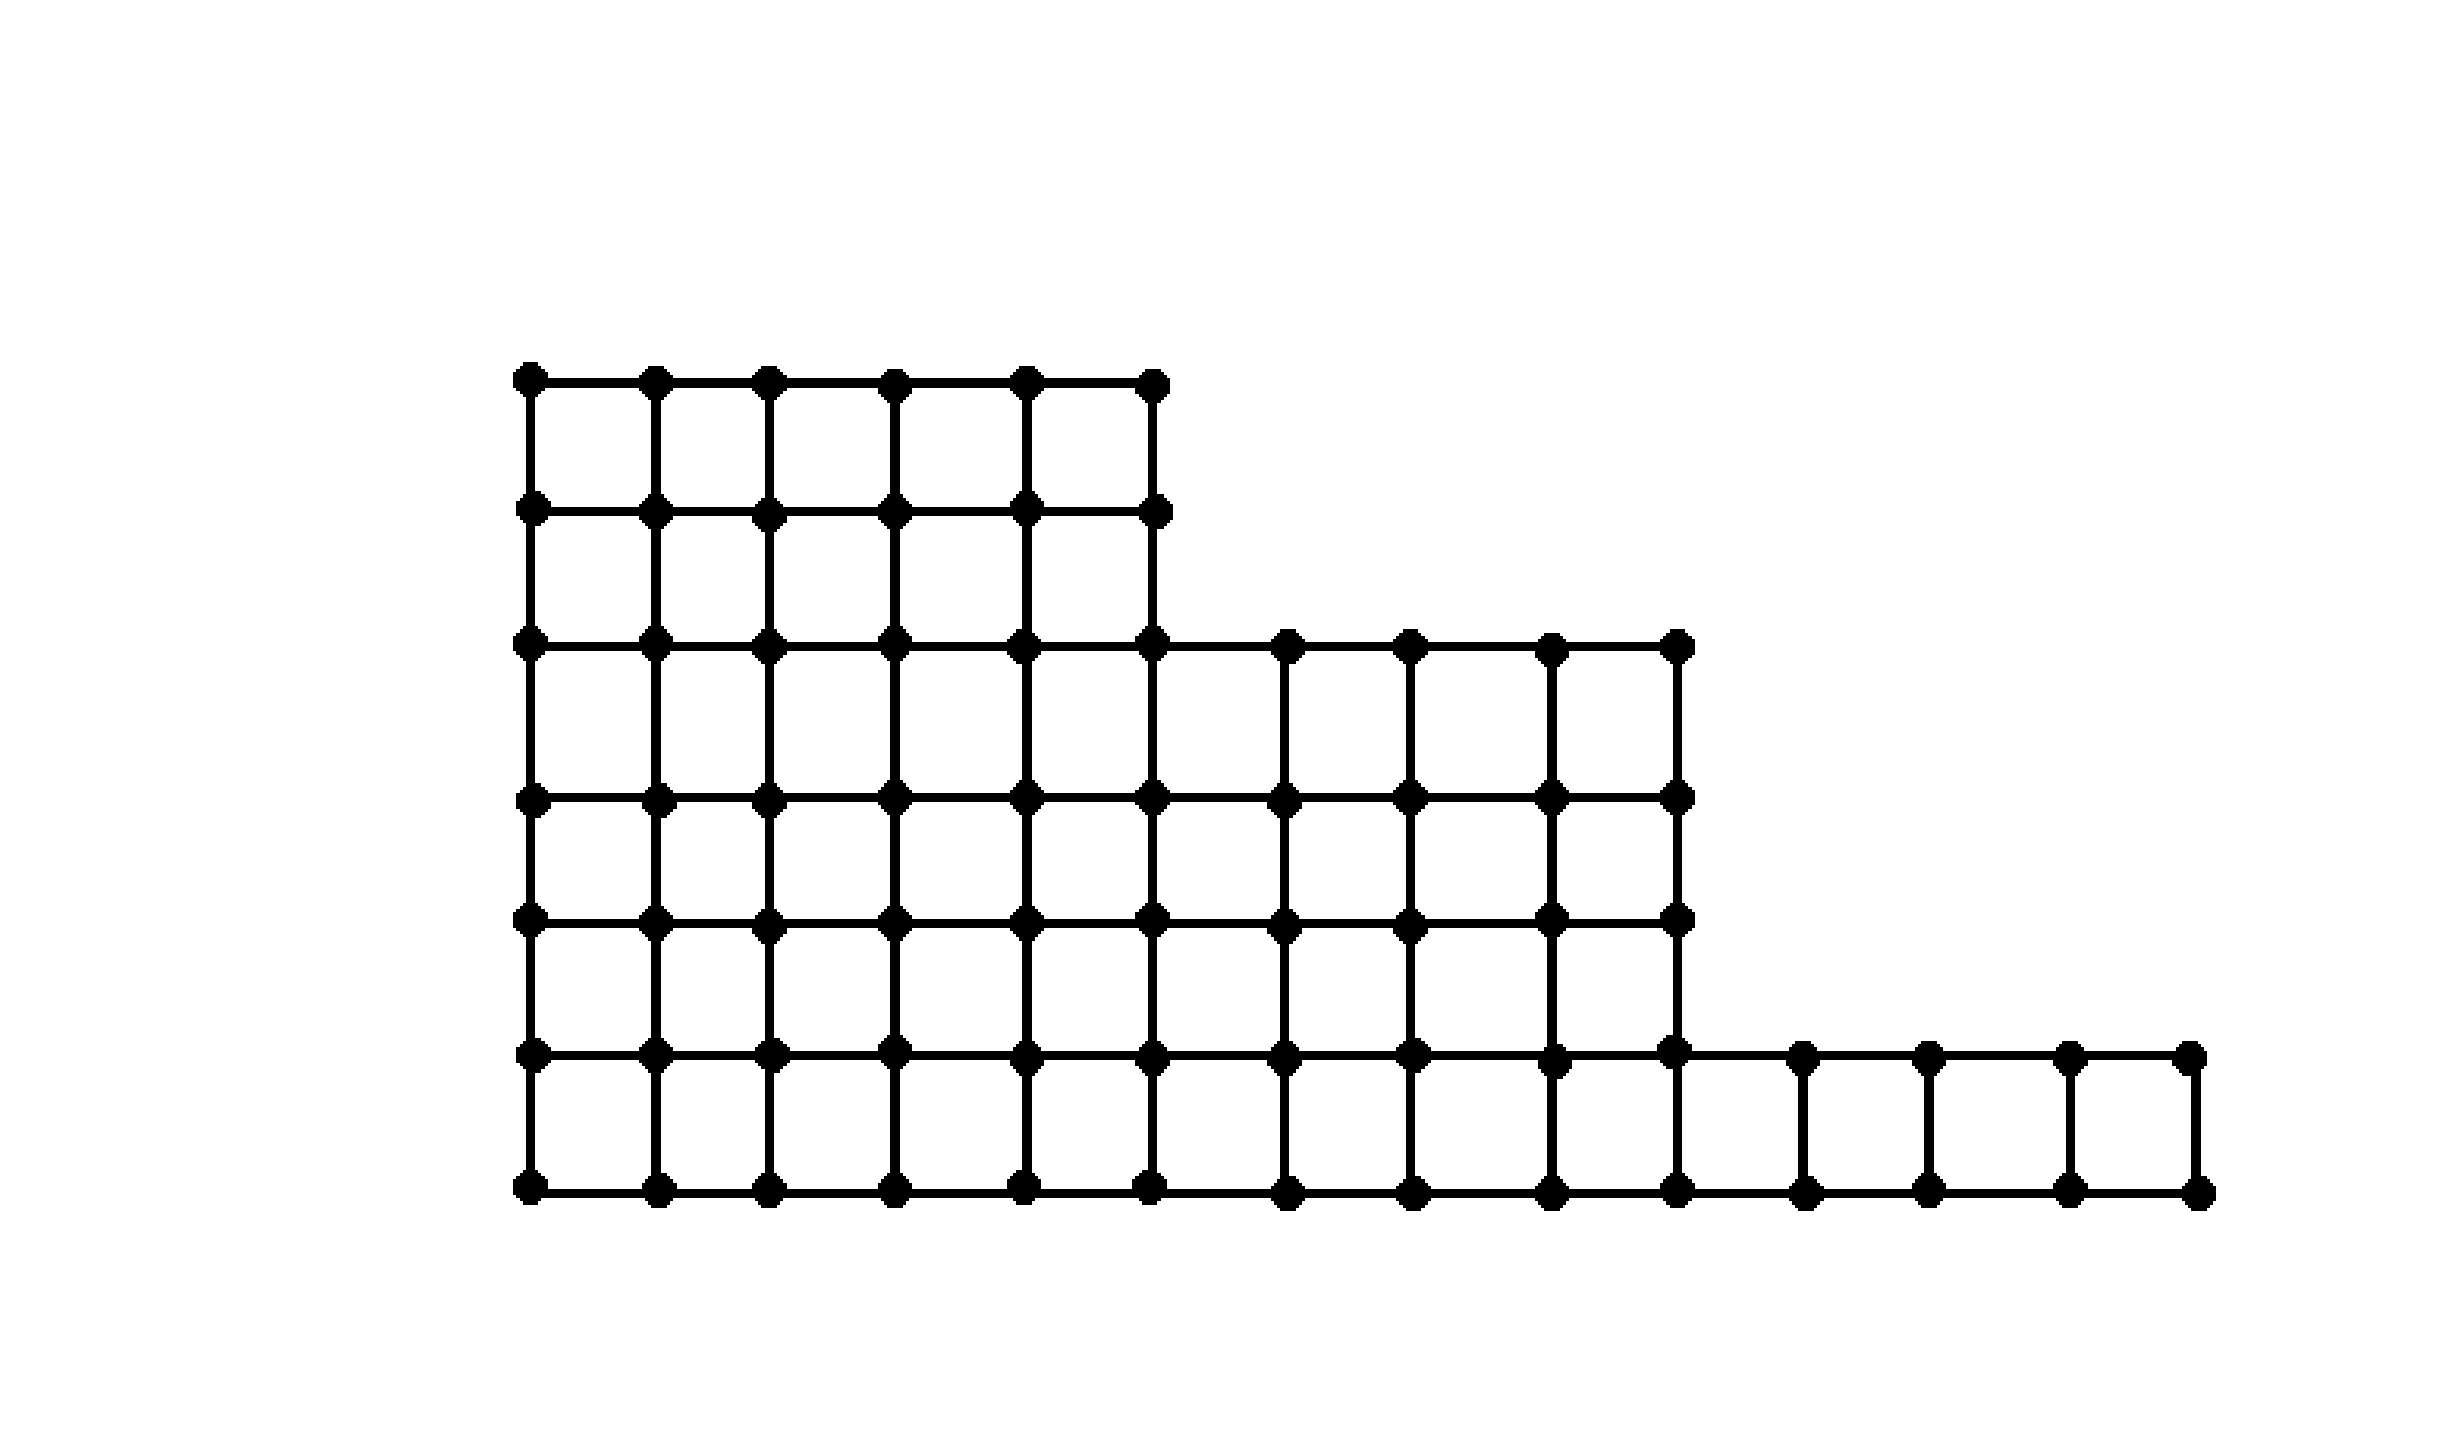
\includegraphics[width=1\linewidth]{images/11111.png} \\ а)}
    \end{minipage}
    \hfill
    \begin{minipage}[h]{0.5\linewidth}
    \center{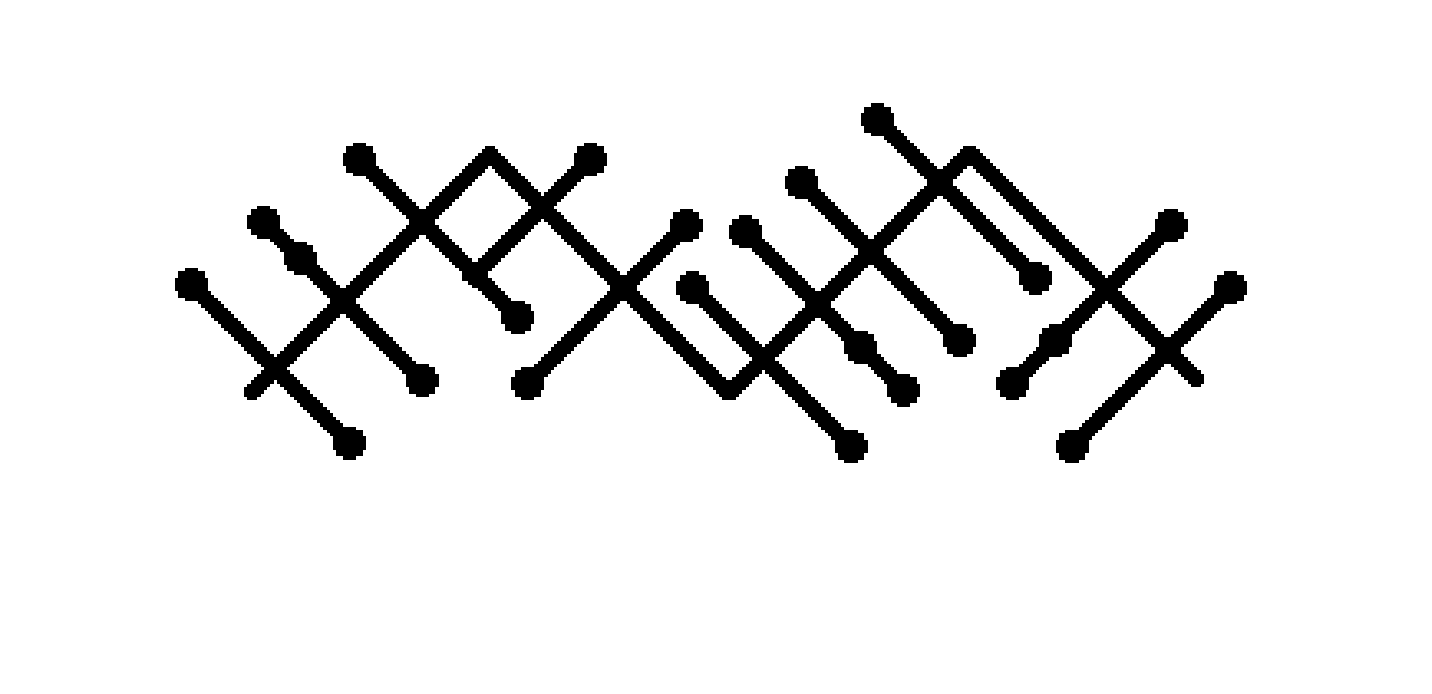
\includegraphics[width=1\linewidth]{images/161616.png} \\ б)}
    \end{minipage}
\caption{Пример регулярной и нерегулярной сетки ЦММ}
\label{fig:6}
\end{figure}
 
\begin{figure}[h]
    \begin{minipage}[h]{0.2\linewidth}
    \center{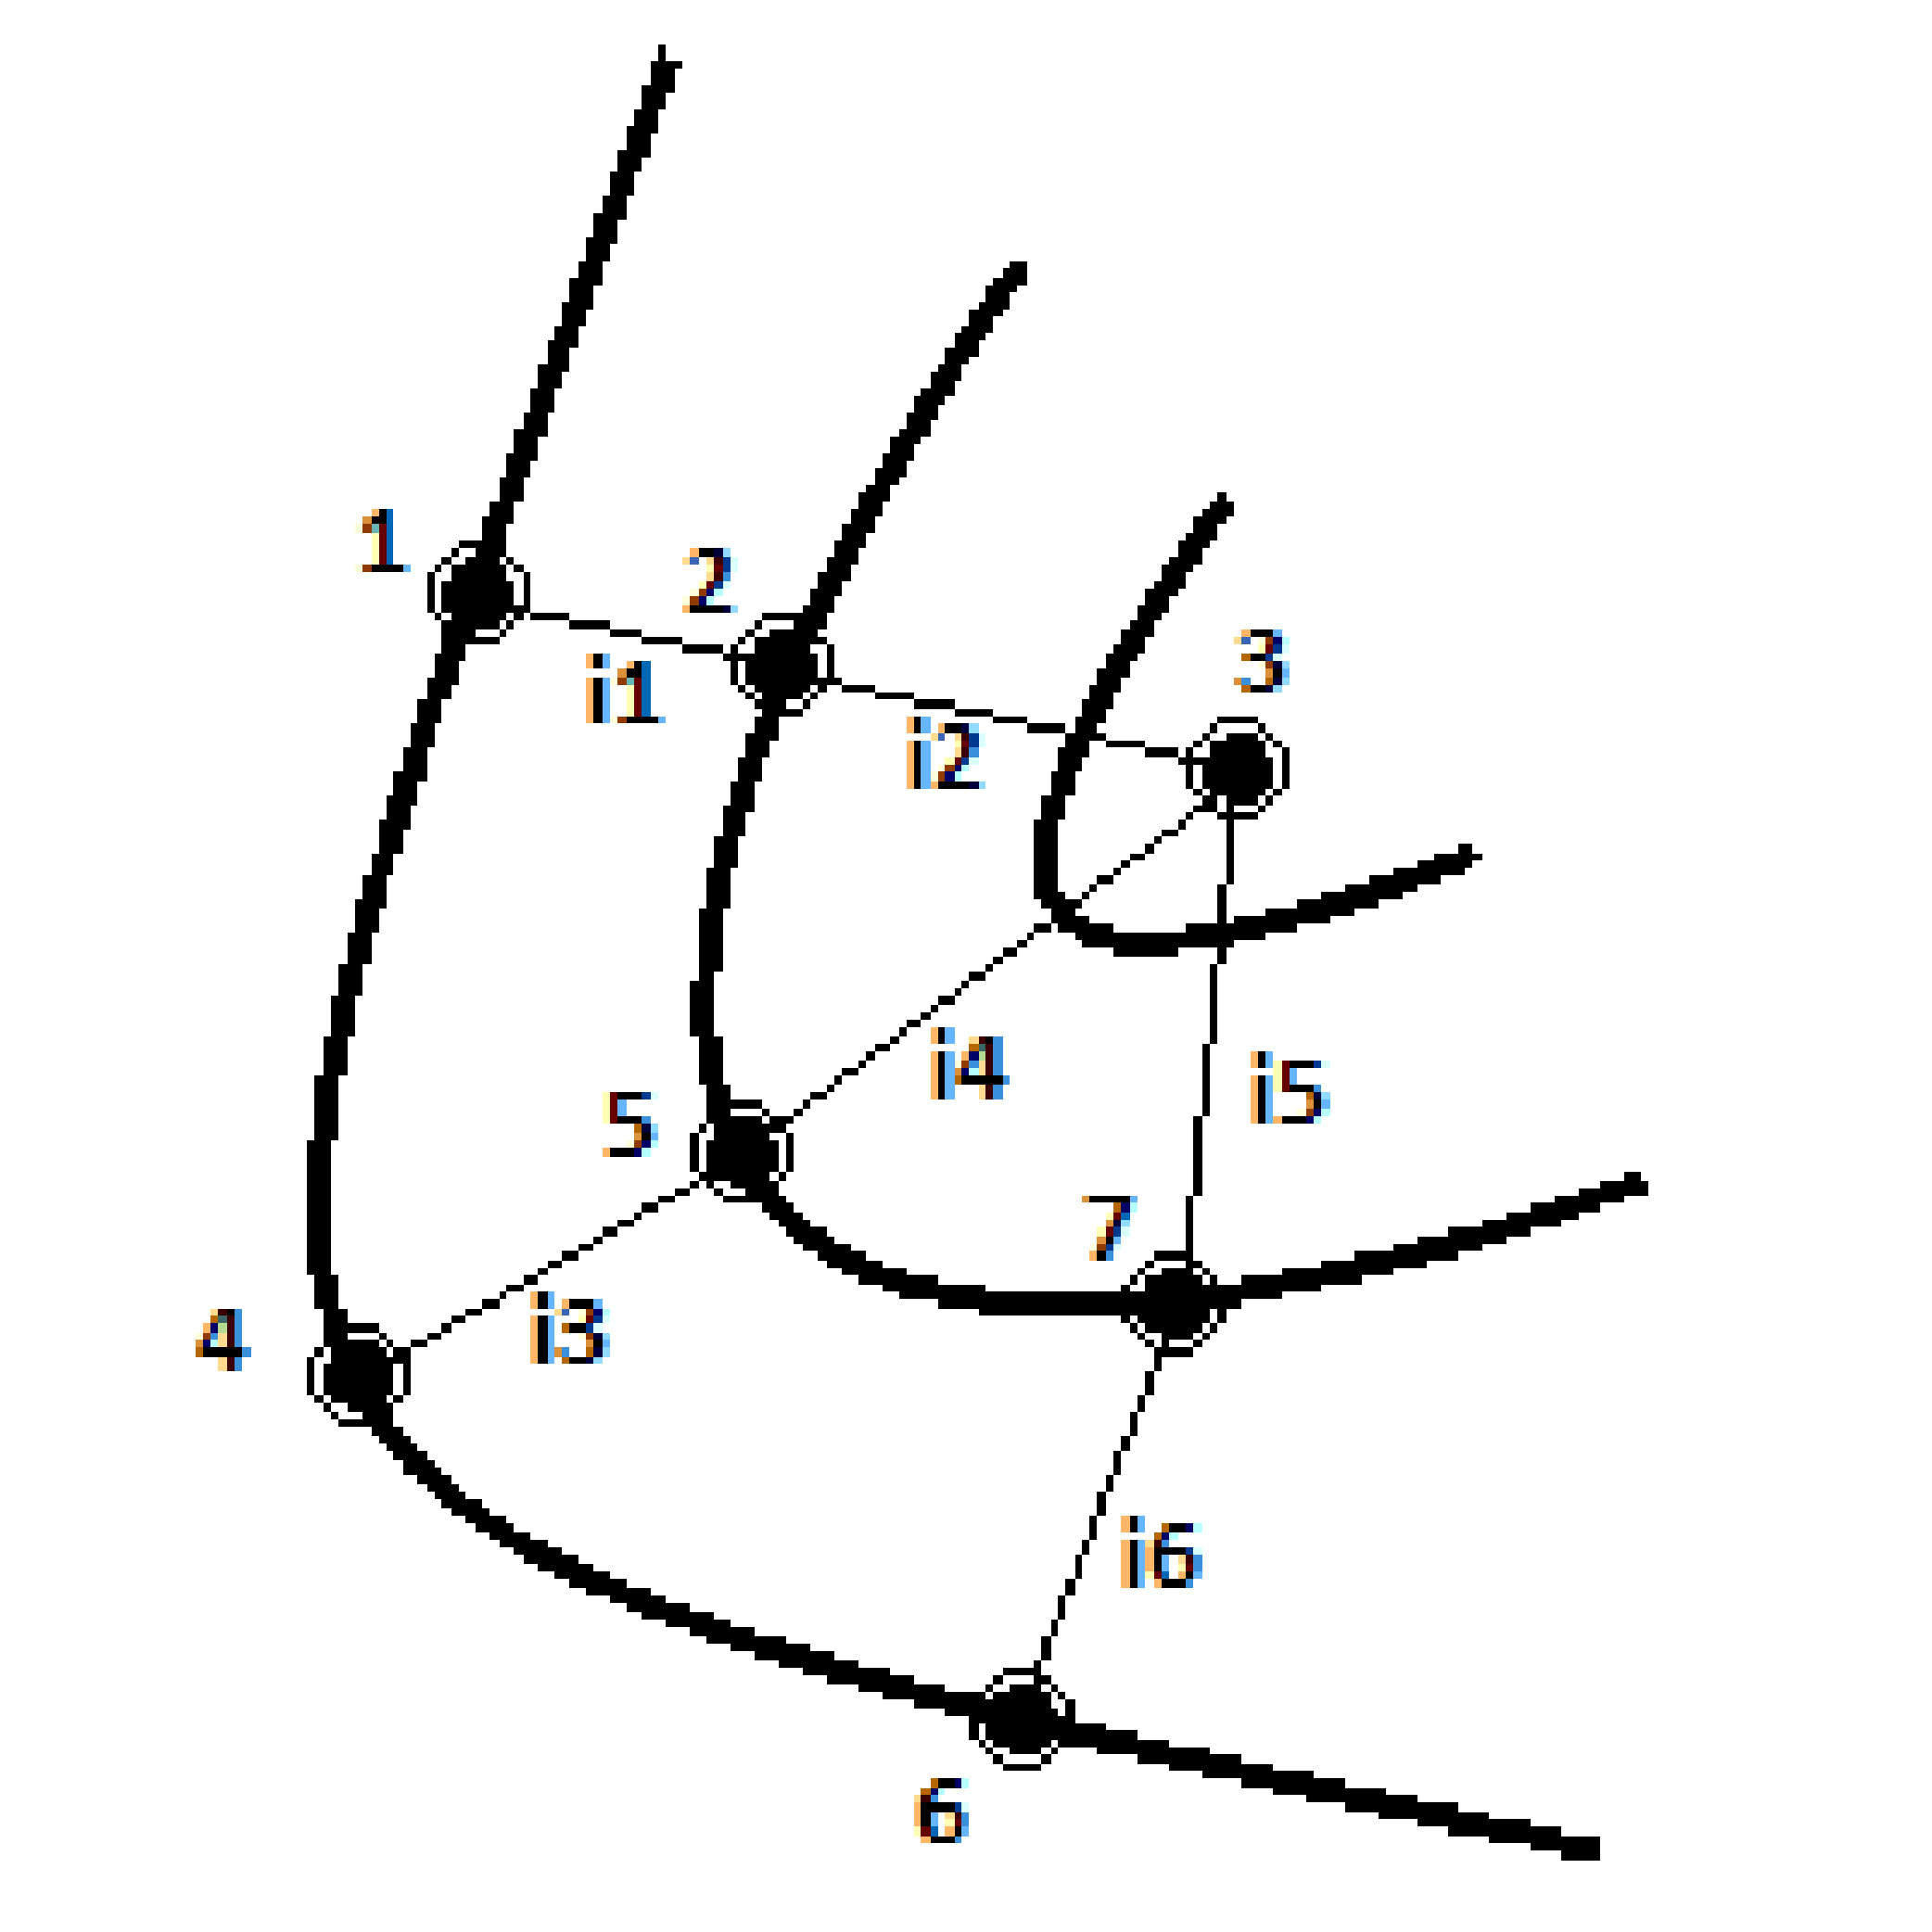
\includegraphics[width=1\linewidth]{images/151515.png} \\ а)}
    \end{minipage}
    \hfill
    \begin{minipage}[h]{0.2\linewidth}
    \center{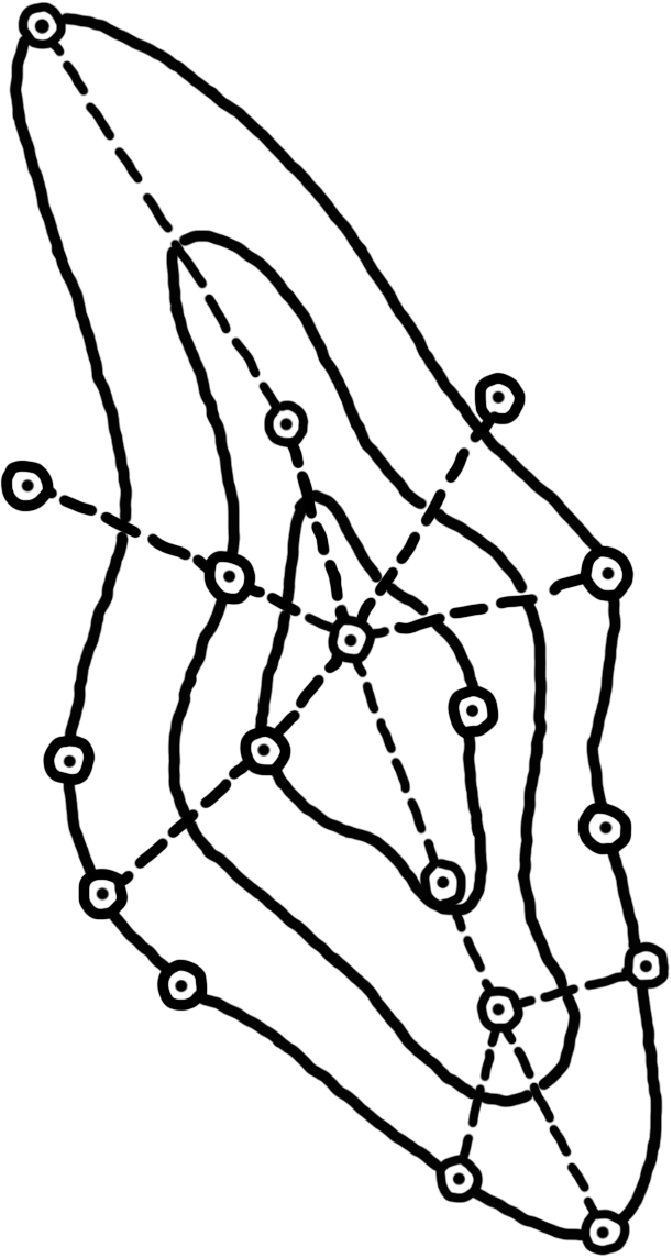
\includegraphics[width=0.8\linewidth]{images/888.png} \\ б)}
    \end{minipage}
    \hfill
    \begin{minipage}[h]{0.2\linewidth}
    \center{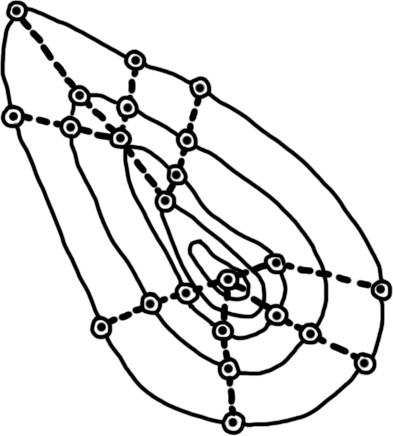
\includegraphics[width=0.8\linewidth]{images/7777.png} \\ в)}
    \end{minipage}
\caption{Примеры сеток структурной ЦММ}
\label{fig:7}
\end{figure}

